
\setcounter{chapter}{7}

\chapter{Individual names for physical objects}
\label{c:gng}
\label{s:grounded-naming-game}


Using the robotic setup from the previous chapter, we will now
investigate what it takes to extend the non-grounded Naming Game from
Chapter \ref{c:naming-game} to a \emph{Grounded Naming
  Game}\footnote{Parts of this chapter were taken from
  \citealp*{steels12grounded-naming-game,loetzsch12grounding,steels12sue}.}.
The main question is: How can a population of robotic agents agree on
a set of \emph{individual names} for physical objects in their
environment?  Naming in this context means assigning different forms
to different individual physical objects in the world -- in the same
way as we give names such as ``John'' to particular persons or
``Alexanderplatz'' to specific places -- and as opposed to labeling
classes of objects (e.g. ``block'' or ``teddy bear''). The key
difference to the non-grounded Naming Game is that the agents do not
have access to shared pre-conceptualized individual objects
(represented by a set of essentially meaningless symbols,
e.g. $\{${\tt obj-1}, {\tt obj-4}, {\tt obj-12}$\}$). Instead, each
agent has to build and maintain conceptual representations that allow
him to classify and individuate different sensory experiences with
respect to which particular physical object they belong to.

 
Populations of agents play the same kind of game as described in
Section \ref{s:language-game} (page \pageref{s:language-game}).  But
instead of using artificial perceptions from a simulated world, agents
perceive physical world scenes through the bodies of two humanoid
robots. Consequently, the \emph{semiotic network} that underlies the
processes of language processing and alignment needs to be
extended. Sensory experiences of objects are classified based on their
similarity to a set of \emph{prototypes}
\citep{edelman98representation}, which are then combined as
\emph{prototypical views} into \emph{individuals}, which are in turn
connected to \emph{names}. We will describe the processes to build and
coordinate these representations in Section
\ref{s:gng-semiotic-networks} below. In addition, heuristics are
needed to decide that two very different sensory experiences (and thus
different conceptual representations) are about one and the same
physical object and two examples of such heuristics are presented in
section \ref{s:gng-heuristics}. Finally, further aspects of the subtle
interplay between language use and the construction of semiotic
networks are discussed in section \ref{s:gng-dynamics}.


\section{Extending the semiotic network}
\label{s:gng-semiotic-networks}

\begin{figure}[t]
  \centerline{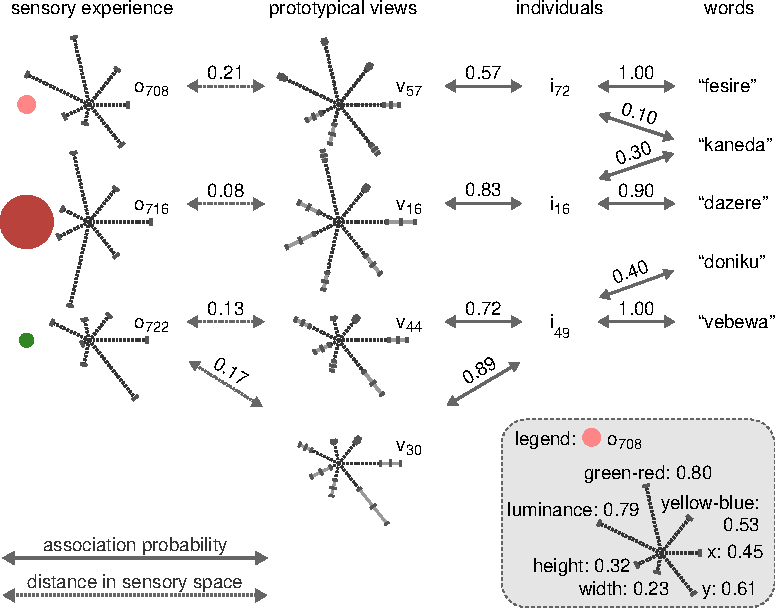
\includegraphics[width=0.8\textwidth]{figures/gng-semiotic-network}}
  \caption{A schematic view of part of a single agent's semiotic
    network. Sensory experiences of objects in the current scene are
    matched with prototypes of past experiences based on distance in
    sensory space. Different prototypical views are connected to
    individuals, which are then linked to words with different
    connection weights. Agents establish semiotic networks and update
    the weights as a side effect of the game. Sensory experiences and
    prototypical views are visualized by their feature vectors. The
    length of each dimension represents the feature mean value and
    standard deviations are indicated with error bars. Note that the
    agents do not memorize sensory experiences -- instead they capture
    their invariant properties in prototypical views.}
  \label{f:gng-semiotic-network}
\end{figure}


The semiotic network maintained by each agent $a$ in the population $P
= \{a_1,a_2,\dots\}$ is a memory of prototypical views, individuals
and names with weighted connections among them (Figure
\ref{f:gng-semiotic-network}). As in all of our non-grounded language
game experiments, they are initially empty and are gradually
constructed by the agents as a side effect of the game. Nodes can be
added or removed and weights between nodes change based on the outcome
of the game.

In order to decide which name to use for a chosen topic, the speaker
determines the prototypical view that best matches the topic and then
finds the most suitable name by tracing his network, each time
following the connection with the highest score. That word is then
transmitted to the hearer, who interprets it by tracing pathways in
his own network but in the other direction. He starts from the name,
looks up the individuals associated with this name, then the possible
prototypical views associated with these individuals, and then the
object that has the highest similarity with one of these prototypical
views. The hearer then points to this object so that the speaker can
give non-linguistic feedback on success or failure. The question how
prototypes, individuals and words are added or removed and how
connection weights in the semiotic network are updated is discussed
below.


\subsection{Capturing object properties with prototypes}
\label{s:gng-prototypes}

In every language game, the speaker and hearer perceive each perceive
a different set of sensory experiences $E~:=~\{e_1,e_2,\dots\}$
constructed by the two robots about the physical objects in a shared
scene from a recorded data set (see section
\ref{s:recording-data-sets}, page \pageref{s:recording-data-sets}). A
sensory experience $e := \langle o(e), \vec{f}(e) \rangle$ is
represented by an object anchor $o$ together with a vector
$\vec{f}~:=~\begin{pmatrix} f_1(e) & \dots & f_7(e)\end{pmatrix}^T$ of
seven continuous visual features {\tt x}, {\tt y}, {\tt width}, {\tt
  height}, {\tt luminance}, {\tt green-red} and {\tt yellow-blue}
scaled into the interval $[0,1]$ (see figure
\ref{f:vision-system-example-scene}, page
\pageref{f:vision-system-example-scene}).


The invariant properties of sensory experiences are captured in terms
of prototypes \citep{edelman95representation,edelman98representation}
and the prototype corresponding to a perception is found using a
nearest neighbor computation. This is motivated by psychological
findings of \cite{rosch73natural,mervis81categorization} who
demonstrated that membership to ``basic level'' categories is
continuous and a function of the similarity to a prototype. As will be
shown below, agents create different prototypes for different views of
the same physical object -- which is why these prototypes are called
prototypical views. Furthermore, agents do not have access to a clear
training set of examples and counter examples that would allow them to
deduce exact distinctions between objects (the machine learning
approach). Instead, each of them has to independently construct his
own inventory of prototypical views over the course of many
interactions with different objects in different contexts.

The prototypical views $V(a)~:=~\{v_1,v_2,\dots\}$ maintained by an
agent $a$ (also dubbed the ``chorus of prototypes'' by
\citealp{edelman95representation}) are modeled as three tuples
$v~:=~\Big{\langle}\vec{f}(v),\sigma\left(\vec{f}(v)\right),\gamma(v)\Big{\rangle}$,
with $\vec{f}(v)$ a vector of feature values as above,
$\sigma\left(\vec{f}(v)\right)$ the variance of feature values (see
below) and $\gamma(v)~\in~[0,1]$ a score reflecting the outcome of
interactions involving that prototypical view. Furthermore, an agent's
semiotic network contains a set of individual
$I(a)~:=\{i_1,i_2,\dots\}$, each of them linked to one or more
prototypical views: $i(a) \subset V(a)$.  A distance function $s$
computing the distance between a sensory experience $e$ and a
prototypical view $v$ is defined as the average difference of feature
values:
$$ s(e,v):=\frac{\sum_{i=1}^{i\leq7}|\left(f_i(e)-f_i(v)\right)|}{7}$$
Many other distance functions such as i.e. Euclidean distance could be
used as well, but since it did not have a significant impact on the
performance of the model, we chose to use the simplest measure. In
order then to determine the best matching prototypical view for a
particular sensory experience $e$, the nearest neighbor
$nn\Big(e,V(a)\Big):E\times V \rightarrow V$ is computed by
calculating the distances $s$ to all prototypical views $V(a)$
maintained by the agent $a$ and selecting the one with the lowest
distance. Similarly, the closest object in a scene for a particular
prototypical view is determined with the nearest neighbor
$nn\Big(v,E(a)\Big):V\times E\rightarrow E$ by computing the distances
to all sensory experiences and also choosing the one with the smallest
distance.

~\\

How are then new prototypes learnt, i.e. how is it decided not to
associate a sensory experience to the closest existing prototypical
view but to create a new one for that object? One possibility would be
to use \emph{sensory distance} itself as a criterion -- when the
distance to the closest prototype is bigger than a fixed threshold,
then a sensory experience would be considered to belong to another
individual object. The problem with this approach is that some
physical objects in the world vary heavily in their appearances,
spanning large areas in sensory space, whereas other objects can be
very close to each other in terms of sensory distance. Therefore, any
fixed threshold would lead to some objects being captured by different
prototypes and some prototypes would cover multiple distinct
objects. A better criterion is \emph{discrimination}: ``only the
comparisons or contrasts between the objects are interesting: if the
world consisted of just one object, it would not really matter how
that object were represented''
\citep[p. 51]{edelman95representation}. An agent observing a scene can
safely assume that the sensory experiences of different physical
objects belong to different individuals and thus must have the closest
distance to different prototypes. If this condition is violated,
i.e. two sensory experiences are associated to the same prototypical
view, then the agent uses one of them as a seed for a new prototypical
view and links it to a newly introduced individual. For example, if
there are two sensory experiences $e_1$ and $e_2$ and two existing
prototypes $v_1$ and $v_2$ such that $s(e_1,v_1) = 0.15$, $s(e_1,v_2)
= 0.1$, and $s(e_2,v_1) = 0.2$, then a new prototype will be built
based on $e_2$ because $v_2$ is the closest prototype to both $e_1$,
and $e_2$ and $e_2$ is further away from $v_2$ than
$e_1$. Consequently, agents have to see objects together in order to
make a difference between them. Suppose for example there is a orange
cube and a red cube of equal size and both objects never occur
together in a scene -- it would be very likely that the agents do not
create different prototypical views for these two objects, treating
the different colors as a natural variance in the appearance of a
single individual object.

\begin{figure}[t]
  \gnuplotfigure{figures/gng-evolution-of-prototype-mean-values}
  \caption{Adjustment of a prototypical view over time. The changing
    feature values of the first prototypical view of the first agent
    in the population are measured in a single series of 25000
    language games and plotted along the x-axis.}
  \label{f:gng-evolution-of-prototype-mean-values}
\end{figure}

As mentioned above, new prototypical views are created from actual
sensory experiences, with the initial prototype features
$\vec{f}(v_{new})$ as a copy of the respective object features
$\vec{f}(e)$. But that particular sensory experience might have been a
rather bad exemplar of the physical object, i.e. it could be that its
features are very different from the average appearance of that
object. An agent seeing an object the first time can not know of
course whether this experience is \emph{prototypical}
\citep{rosch75family-resemblances} for that object (sometimes also
called \emph{representative} or \emph{central}). That's why prototypes
have to get adjusted later on to better reflect the distributional
properties defining that physical object. In every interaction in that
a prototypical view $v_t$ at time $t$ is the nearest neighbor to a
sensory experience $e$, the prototype feature values $\vec{f}(v_t)$
and variance $\sigma\left(\vec{f}(v_t)\right)$ are recursively updated
for all features $f_i$:
\begin{eqnarray*}f_i(v_t) & = & \alpha \cdot f_i(v_{t-1}) + \left(1 - \alpha\right) \cdot f_i(e) \\
  \sigma\left(f_i(v_t)\right) & = & \alpha \cdot
  \left(\sigma\left(f_i(v_{t-1})\right) + \left(f_i(v_t) -
      f_i(v_{t-1})\right)^2\right) + \left(1 - \alpha\right) \cdot
  \left(f_i(e) - f_i(v_t)\right)^2\end{eqnarray*} with $\alpha=0.995$
being a stability factor, weighting the impact of new experiences.
Especially in the beginning when not all physical objects have been
encountered yet it might happen that prototypical views span multiple
physical objects in sensory space. Therefore -- as a conservative
strategy -- feature values are only shifted when the distance between
the experience and the prototype is not too far away from the standard
deviation of that feature: $|f(o)-f(v)|-\sigma^2\left(f(v)\right) <
\epsilon$, with $\epsilon = 0.1$ (this is also the only reason why
prototype feature variances are maintained). Figure
\ref{f:gng-evolution-of-prototype-mean-values} gives an example for
this adjustment process. It is shown how the feature values of a
single prototypical change over time, stabilizing towards the
end. Apparently the sensory experience used to create this particular
prototype was less representative for that object, especially in the
{\tt x}, {\tt width} and {\tt height} features, which get adjusted the
most in the beginning.

\begin{measure}[b]{Object similarity}{m:object-similarity}
  The distance $s$ between the sensory experiences of speaker $E(sp)$
  and hearer $E(h)$ of the objects in the current scene is computed
  and averaged over the objects in the scene: $$\text{object
    similarity} :=
  \frac{\sum_{i=1}^{i\leq|E|}s\left(e_i(sp),e_i(h)\right)}{|E|}$$ The
  correspondence between the objects in the two world models is
  established by letting the speaker point at each object and the
  hearer determining the respective sensory experience by interpreting
  the pointing (see section \ref{s:scaffolding-social-skills}, page
  \pageref{s:scaffolding-social-skills}).
\end{measure}

\begin{measure}[b]{Prototype similarity}{m:prototype-similarity}
  Prototype similarity measures the average sensory distance between
  the prototypical views associated by the speaker $sp$ and hearer $h$
  to the objects in the current scene $E(sp)$ and $E(h)$:
  $$\text{prototype similarity}
  ~:=\frac{\sum_{i=1}^{i\leq|E|}s\left(nn\left(e_i(sp),V(sp)\right),\
      nn\left(e_i(h),V(h)\right)\right)}{|E|}$$ Correspondence between
  the sensory experiences of speaker and hearer is established by
  pointing. Results are averaged over the last 250 interactions.
\end{measure}

\begin{figure}[t]
  \gnuplotfigure{figures/gng-prototype-similarity}
  \caption{The average similarity between the prototypical views used
    by the speaker and hearer for the objects in the current scene
    (measure \ref{m:prototype-similarity}) are shown for agents with
    and without adjustment. For comparison, the average sensory
    distance between the objects in the contexts of speaker and hearer
    (measure \ref{m:object-similarity}) is plotted too. }
  \label{f:gng-prototype-similarity}
\end{figure}

As a result, the agents independently self-organize their prototypical
views in a clustering process, exploiting structure in the world
\citep{rosch76basic} that is observed through the statistical
distributions of features in sensory experiences. Note that our model
does not depend on the choice of this particular mechanism for
maintaining prototypes -- other techniques such as for example Radial
Basis Function networks \citep{poggio90networks} or Kohonen maps
\citep{kohonen82self-organized} could be used equally well. Figure
\ref{f:gng-prototype-similarity} shows how the sensory distance $s$
between the prototypes used by speaker and hearer for the same object
changes over time. When prototype features are not adjusted, then the
average distance decreases a bit in the beginning (because more
prototypical views get learnt, automatically decreasing the distance
between prototypes) and remains constant at around 0.095, which is
even higher than the average distance between the sensory experiences
of speaker and hearer ($\approx$ 0.085). Otherwise -- when feature
values are adjusted -- the similarity between prototypes further
decreases to approach $\approx$ 0.06. The average distance does not
reach zero because the two agents can have significantly different
perceptions of objects -- an agent that (unnaturally) would have
access to the perceptions of both robots for a scene would not
necessarily associate the same prototypical view to the different
sensory experiences for the same physical object, as discussed further
down.

\begin{figure}[t]
  \gnuplotfigure{figures/gng-evolution-of-prototype-scores}
  \caption{Evolution of a single agent's prototype scores. The scores
    of all prototypical views in the semiotic network of agent 1 out
    of a population of 10 agents are recorded in a single run of 25000
    interactions and plotted along the x-axis.}
  \label{f:gng-evolution-of-prototype-scores}
\end{figure}

Even with these adjustment mechanisms it is not guaranteed that a
prototypical view is connected exclusively to the sensory experiences
of the same physical object. In fact it happens quite often that
prototypes find a niche in the sensory space where there are close to
different objects. However, if this is the case, then the words
associated to these prototypical views via connected individuals are
also less successfully used in language games because the hearer
interpreting them more often points to the wrong object. This can be
used as a criterion to further shape an agent's semiotic network:
After each successful interaction, both speaker and hearer increase
the score $\gamma(v)$ of the prototype $v$ that they associated to the
topic by the fixed delta of 0.025, and in each interaction that failed
they decrease the score by the same amount. Prototypes that reach a
score of 0 or below are removed from the agent's semiotic network,
together with the individuals and words connected to them (unless they
still have links to other prototypes/ individuals in the
network). Furthermore, in order to ``forget'' prototypes that occupy
regions in the sensory space where they are almost never used, the
scores of all prototypes are reduced in each interaction by a constant
decay factor of $0.01 / |V(a)|$. Figure
\ref{f:gng-evolution-of-prototype-scores} illustrates these
dynamics. Most prototypical views immediately reach a score of 1, but
some of them fail to be consistently used in successful interactions
so that a few prototypes eventually get deleted.


\subsection{Linking individuals to words}
\label{s:gng-lexicon}

The words in a semiotic network connect individuals to forms. Besides
that, the lexicon representations are exactly the same as in the
non-grounded Naming Game (Chapter \ref{c:naming-game} on page
\pageref{c:naming-game}). An agent's lexicon $L(a)$ is a set of words,
represented by three tuples $w := \langle i, f, \gamma \rangle \in
I(a)\times{\cal F}\times \mathbb{R}$. Each word associates an
individual $i \in I(a)$ to a form $f \in {\cal F}$ with an association
weight $\gamma$ representing the agent's confidence in that
association. ${\cal F}$ is the set of possible word forms and $\gamma$
is a real value with $0 \leq \gamma \leq 1$.

A speaker tracing his semiotic network in search for a name for the
chosen topic first determines the closest prototype and the linked
individual and then finds the word in his lexicon connected to this
individual that has the highest score. When a speaker does not have a
name for an individual $i \in I(a)$, he generates a new unique name
$f_{new}$ by making a random combination of syllables and adds the
association $\langle i,f_{new},\gamma_{init} \rangle$ to his semiotic
network with an initial weight $\gamma_{init}=0.5$. A hearer
encountering a new name will signal a communicative failure, the
speaker then points to the intended object and the hearer determines
the corresponding individual. A new association between that
individual and the name heard is added to the lexicon with the same
initial score of $0.5$. In order to reflect how well a name is
conventionalized in the population, both speaker and hearer increase
the weight of the association used by $\Delta\gamma_{succ}=0.1$ after
a successful language game and decrease the word score by
$\Delta\gamma_{fail}=0.1$ in unsuccessful interactions. Furthermore,
synonyms (associations of the same individual to different forms) are
dampened using lateral inhibition: After each successful interaction
both involved agents decrease the weights of all associations with the
same individual but different forms by $\Delta\gamma_{inhib}=0.2$.

\begin{figure}[t]
  \gnuplotfigure{figures/gng-number-of-words-and-synonyms-and-homonyms}
  \caption{Lexicon size and the average number of synonyms and
    homonyms averaged over all 10 agents of the population. Error bars
    are standard deviations over 10 repeated experimental runs of
    25000 interactions each. See measures \ref{m:lexicon-size},
    \ref{m:synonymy} and \ref{m:homonymy} (page
    \pageref{m:lexicon-size} ff.)}
  \label{f:gng-number-of-words-and-synonyms-and-homonyms}
\end{figure}

Agents start with initially empty lexicons and since words are learnt
in local interactions between randomly chosen members of the
population, many different word forms for the same physical objects
are created independently by different speakers. In a population of 10
agents, on average two different individuals get associated to a form
in the first few hundred interactions (see figure
\ref{f:gng-number-of-words-and-synonyms-and-homonyms}). Lateral
inhibition quickly reduces synonymy, eventually decreasing and
stabilizing the average number of associations in each agent's
lexicon. However -- different from the non-grounded Naming Game --
independent creation of word forms is not the only cause for the
creating of synonyms. As discussed above, different agents develop
very different sets of prototypes and thus there is no guarantee that
a name is used exclusively for the sensory experiences of one
particular physical object -- even though a hearer adopting a novel
word knew the object that was intended by the speaker through
pointing. It might for example happen that one speaker has a
suboptimal prototypical view that gets associated to the sensory
experiences of two different physical objects in different sensory
contexts. Therefore the word connected to that prototype and linked
individual would be used by the agent for different physical objects
(note that his is not homonymy because that name is connected to only
one individual and prototype). Another hearer that uses the name for
only one physical object (because the linked prototypical view is
associated to only one object in the world) might happen to interact
with the agent. When the speaker uses the word for another object than
understood by the hearer, then the communication will fail and the
speaker will point to the object intended, eventually causing the
hearer to adopt a synonym for the individual linked to that object
(given that he knew already another name for that individual).
Consequentially, the average number of synonyms in the agents'
lexicons never completely reaches zero (compare to Figure
\ref{f:ng-synonymy+coherence} on page
\pageref{f:ng-synonymy+coherence}) but remains at a level of about 0.1
as shown in Figure
\ref{f:gng-number-of-words-and-synonyms-and-homonyms}.

\begin{figure}[t]
  \gnuplotfigure{figures/gng-evolution-of-word-scores}
  \caption{A single agent's lexicon as it changes over time. For each
    word form in the lexicon of the first agent the word scores of all
    associations involving that form are averaged and plotted along
    the x-axis (in a single run). The population size for this graph
    is limited to five in order to restrict the number of word forms.}
  \label{f:gng-evolution-of-word-scores}
\end{figure}

Prototypical views associated to different physical objects is also
one of the two causes for homonyms, i.e. different individuals
connected to the same name (a phenomenon also absent in the
non-grounded Naming Game). The hearer in the example above will
connect the name to both the individual that was initially understood
and to the individual connected to the object pointed at. A second
cause for homonymy is that agents can associate multiple prototypical
views to the same physical object as explained below. A hearer then
might adopt the same name to different individuals linked to the same
object. On average every 10th name an agent's lexicon is homonymous
(see figure \ref{f:gng-number-of-words-and-synonyms-and-homonyms}).


The suboptimal interrelation between individuals and physical objects
and the fact that prototypical views and individuals can get removed
from an agent's semiotic network are responsible for a much higher
degree of change in the lexicon than in the non-grounded Naming Game
(see Figure \ref{f:gng-evolution-of-word-scores} compared to
Figure \ref{f:ng-word-scores} on page
\ref{f:ng-word-scores}). Although most words are created and adopted
in the first few hundred interactions and quickly aligned trough
lateral inhibition, there are some words that enter the lexicon much
later and even consistently successful words are sometimes used in
interactions that fail (resulting in their scores going down from 1
and then quickly up again).




\subsection{Similarity is not enough}

\begin{figure}[p]
  \rotatebox{90} {
\renewcommand{\arraystretch}{1.3}{
  \begin{tabular}{@{}p{0.5cm}lp{1.2cm}p{1.2cm}p{1.2cm}llp{1.2cm}p{1.2cm}p{1.2cm}c@{}}
    \# & speaker & topic speaker & prototypical view speaker & individual speaker & utterance & hearer & individual hearer & prototype hearer & topic hearer & success? \\
    \hline
    500 & agent 3 & \texttt{obj-144} & \texttt{v-1} & \texttt{i-1} & \textit{``vomegi''} & agent 1 & \texttt{v-26} & \texttt{i-26} & \texttt{obj-147} &  yes \\
    501 & agent 5 & \texttt{obj-148} & \texttt{v-122} & \texttt{i-122} & \textit{``zedaba''} & agent 4 & \texttt{} & \texttt{} & \texttt{} &  no \\
    502 & agent 5 & \texttt{obj-147} & \texttt{v-101} & \texttt{i-101} & \textit{``fimuzu''} & agent 4 & \texttt{v-45} & \texttt{i-45} & \texttt{obj-144} &  yes \\
    503 & agent 1 & \texttt{obj-138} & \texttt{v-98} & \texttt{i-98} & \textit{``wifote''} & agent 10 & \texttt{v-59} & \texttt{i-59} & \texttt{obj-139} &  yes \\
    504 & agent 1 & \texttt{obj-136} & \texttt{v-28} & \texttt{i-28} & \textit{``rebama''} & agent 10 & \texttt{v-103} & \texttt{i-103} & \texttt{obj-137} &  yes \\
    505 & agent 4 & \texttt{obj-163} & \texttt{v-107} & \texttt{i-107} & \textit{``tasuse''} & agent 6 & \texttt{v-53} & \texttt{i-53} & \texttt{obj-159} &  yes \\
    506 & agent 4 & \texttt{obj-162} & \texttt{v-47} & \texttt{i-47} & \textit{``bibeno''} & agent 6 & \texttt{v-31} & \texttt{i-31} & \texttt{obj-153} &  yes \\
    507 & agent 1 & \texttt{obj-152} & \texttt{v-84} & \texttt{i-84} & \textit{``birupu''} & agent 6 & \texttt{} & \texttt{} & \texttt{} &  no \\
    508 & agent 1 & \texttt{obj-157} & \texttt{v-29} & \texttt{i-29} & \textit{``bibeno''} & agent 6 & \texttt{v-31} & \texttt{i-31} & \texttt{obj-153} &  yes \\
    509 & agent 4 & \texttt{obj-173} & \texttt{v-68} & \texttt{i-68} & \textit{``tavoke''} & agent 2 & \texttt{v-58} & \texttt{i-58} & \texttt{obj-177} &  yes \\
    510 & agent 4 & \texttt{obj-175} & \texttt{v-107} & \texttt{i-107} & \textit{``tasuse''} & agent 2 & \texttt{} & \texttt{} & \texttt{} &  no \\
    511 & agent 6 & \texttt{obj-43} & \texttt{v-49} & \texttt{i-49} & \textit{``fepaka''} & agent 4 & \texttt{v-54} & \texttt{i-54} & \texttt{obj-52} &  yes \\
    512 & agent 6 & \texttt{obj-44} & \texttt{v-105} & \texttt{i-105} & \textit{``tunite''} & agent 4 & \texttt{} & \texttt{} & \texttt{} &  no \\
    513 & agent 9 & \texttt{obj-9} & \texttt{v-39} & \texttt{i-39} & \textit{``vomegi''} & agent 7 & \texttt{v-23} & \texttt{i-23} & \texttt{obj-9} &  yes \\
    514 & agent 9 & \texttt{obj-3} & \texttt{v-37} & \texttt{i-37} & \textit{``kogise''} & agent 7 & \texttt{v-108} & \texttt{i-108} & \texttt{obj-6} &  yes \\
    515 & agent 5 & \texttt{obj-148} & \texttt{v-87} & \texttt{i-87} & \textit{``vubeta''} & agent 6 & \texttt{v-90} & \texttt{i-90} & \texttt{obj-152} &  yes \\
    516 & agent 5 & \texttt{obj-152} & \texttt{v-92} & \texttt{i-92} & \textit{``wifote''} & agent 6 & \texttt{v-17} & \texttt{i-17} & \texttt{obj-155} &  no \\
    517 & agent 4 & \texttt{obj-179} & \texttt{v-107} & \texttt{i-107} & \textit{``tasuse''} & agent 7 & \texttt{} & \texttt{} & \texttt{} &  no \\
    518 & agent 4 & \texttt{obj-182} & \texttt{v-83} & \texttt{i-83} & \textit{``zozeri''} & agent 7 & \texttt{v-19} & \texttt{i-19} & \texttt{obj-177} &  yes \\
    519 & agent 7 & \texttt{obj-147} & \texttt{v-79} & \texttt{i-79} & \textit{``gudute''} & agent 4 & \texttt{} & \texttt{} & \texttt{} &  no \\
  \end{tabular}}



%%% Local Variables: 
%%% mode: latex
%%% TeX-master: "../phdbook"
%%% End: 
}
  \caption{Overview of 20 consecutive interactions from game 500
    on. It shows the agents that are interacting, the topic picked by
    the speaker, the prototypical views and individuals used by both
    agents, the utterance formed, the topic understood by the hearer
    (when successfully parsed) and whether the agents reached
    communicative success.}
  \label{f:gng-trace}
\end{figure}



With all the introduced mechanisms for creating and maintaining
semiotic networks the agents are able to establish successful
communication systems. As illustrated by the example interactions in
Figure \ref{f:gng-trace} (and different from all experiments in
simulated environments in Chapters \ref{c:naming-game} and
\ref{c:gg}), they do so by sharing not any mental representations
other than word forms -- perceptions, prototypical views and
individuals are internal to the semiotic networks of each agent. Note
ids of objects can reoccur in later interactions (for example the
objects \texttt{obj-144} and \texttt{147} are perceived both by the
agents in interaction 500 and 502). This is due to the nature of
embodied perception as being from a recorded data set of robotic
perceptions (see Section \ref{s:recording-data-sets}). However, these
ids are for illustration purposes only. They are not processed or
stored by the interacting agents, even not for pointing.

\begin{figure}[t]
  \gnuplotfigure{figures/gng-results-without-heuristics}
  \caption{Commun\-icative success (measure
    \ref{m:communicative-success}) and inventory sizes (measures
    \ref{m:lexicon-size}, \ref{m:number-of-prototypical-views} and
    \ref{m:number-of-individuals}) in a population of 10 agents
    playing 25000 language games. Error bars are standard deviations
    over 10 repeated runs of 25000 interactions each.  }
  \label{f:gng-results-no-heuristics}
\end{figure}

\begin{measure}[b]{Number of prototypical views}{m:number-of-prototypical-views}
  The number of prototypical views in each agent's semiotic network is
  counted and averaged over the number of agents in the population:
  $\text{number of prototypical views} :=
  \sum_{i=1}^{i\leq|P|}|V(a_i)|\ /\ |P|$. Values are averaged over the
  last 100 interactions.
\end{measure}

\begin{measure}[b]{Number of individuals}{m:number-of-individuals}
  The number of individuals in each agent's semiotic network is
  counted and averaged over the number of agents in the population:
  $\text{number of individuals} := \sum_{i=1}^{i\leq|P|}|I(a_i)|\ /\
  |P|$. Values are averaged over the last 100 interactions.
\end{measure}


Figure \ref{f:gng-results-no-heuristics} shows
the overall dynamics in a population of 10 agents playing 25000
language games. After about 2500 interactions (which means that on
average each agent took part in 500 games) they are able to
successfully draw the attention of the hearer to the intended object
and later on communicative success rises to above 95$\%$. The number
of prototypical views (and the equal number of individuals --
individuals are automatically created and linked to newly introduced
prototypes) rises quickly in the beginning and then more slowly toward
the end (because agents still see new objects and because they
optimize their inventories based on communicative success) to finally
reach a number of about 17. The lexicon size peaks in the beginning
and later on approaches the number of individuals, with out reaching
it due to a stable amount of synonyms and homonyms in the lexicon.

However, there are only ten different physical objects in the world
(see section \ref{s:recording-data-sets}, page
\pageref{s:recording-data-sets}), but the agents associate 17
individuals to them, 1.7 on average. This is because objects in the
world can drastically vary in their appearances -- both over time and
within the same scene when viewed by the two robots from different
angles. For example a red bar can look very narrow when standing and
wide when lying down. And colors of objects can be different from
different viewing angles. As a result, different prototypes are
created for the sensory experiences of the same object in different
orientations or viewing angles because the similarity between these
views is lower than to other prototypes (a standing red block could be
more similar to a standing orange block than to the same red block
lying down).

Similarity based on prototypes is thus not enough for creating
individual concepts and names about physical objects that often change
their view. The language self-organized by agents endowed with the
mechanisms discussed so far cannot be interpreted as a set of
individual names but rather as words naming different views of
objects. Further mechanisms are therefore needed to establish object
identity.

\section{Heuristics for establishing object identity}
\label{s:gng-heuristics}

The sensory experiences of objects themselves don't reveal whether
they belong to the same or different individuals. For example it could
be that perceptions of something big and red and something small and
red are about the same physical object, and at the same time
experiences of big blue and small blue things could belong to
different individuals. However, heuristics that exploit other
knowledge about the interaction with objects can be employed and we
demonstrate how two of them can help the agents to optimize their
semiotic networks in order to establish object identity.

The ``object tracking'' heuristic makes the assumption that if an
agent observes how an object changes its appearance, he can infer that
the resulting different views must be about the same individual. For
example if see somebody painting his red car in green, we will know
that it is still the same object. And we have no problems following
the plot of a fairy tale in which a frog turns into a prince as long
we can witness this transformation. Second, the ``same name''
heuristic assumes that objects that are referred to with the same name
must be the same individual. Imagine seeing someones child and
learning her the name and much later meeting a person with the same
name. Even though the child grew much taller, wears different clothes,
has different hairstyle etc., we will assume that it is the same
person. The number of heuristics employed by humans is without doubt
much bigger. For example we sometimes can assume that things observed
in a fixed location are the same, that the dog being frequently walked
by our neighbor is always the same dog although we have difficulties
discriminating dogs, and so on.


\subsection{Observing objects change}
\label{s:object-persistence}

\begin{figure}[t]
  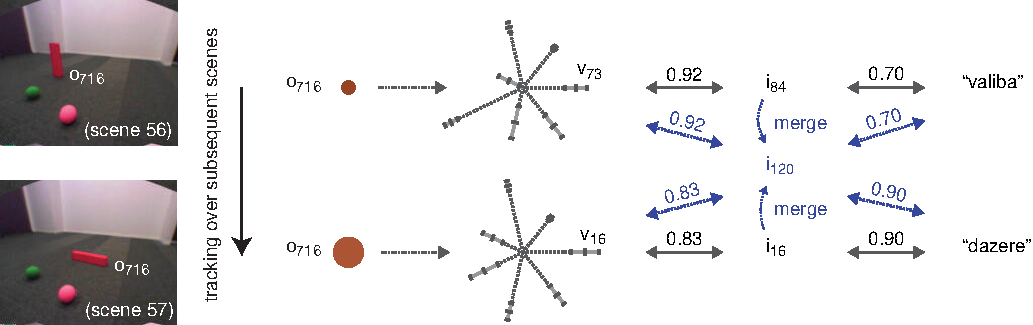
\includegraphics[width=1\textwidth]{figures/gng-heuristic-object-persistence}
  \caption{The 'object tracking' heuristic. The red bar changes its
    appearance from one scene to the next, resulting in different
    prototypical views being associated with the respective sensory
    experiences. The vision system is able to track the object during
    the movement via the same anchor $o_{716}$, making it possible to
    assume that the two prototypical views are about the same physical
    object and thus their connected individuals can be merged.}
  \label{f:gng-heuristic-object-persistence}
\end{figure}

The vision system is able to track objects over space and time as
detailed in see section \ref{s:vision-system} (page
\pageref{s:vision-system}). Figure
\ref{f:gng-heuristic-object-persistence} shows how the sensory
experiences for an object that changes its appearance from one scene
to the next gets associated to different prototypical views of a
particular agent: The nearest neighbor of $o_{716}$ is $v_{73}$
(linked to $i_{84}$) in scene 56 and $v_{16}$ (linked to $i_{16}$) in
scene 57. Knowing that these different perceptions are about the same
physical object (established through the anchor $o_{716}$), the agent
can assume that the two individuals $i_{84}$ and $i_{16}$ must be
about the same object and thus can be ``merged''. The semiotic network
of the agent is then rearranged by introducing a new individual
$i_{120}$, linking $i_{120}$ with all words or prototypical views that
were connected to the original individuals and finally removing
$i_{84}$ and $i_{16}$ from the network. The previously independent
names ``valiba'' and ``dazere'' are now synonyms and later
interactions will determine what the winning name for the new
individual is. In order to avoid merging prototypes that have not
found their final position in sensory space yet, only individuals
views that were independently used in successful interactions are
merged -- the weights of all links to the individuals in questions
(both the scores of prototypes and words) have to be higher than a
threshold value of 0.9. Finally, it is worth mentioning how the agents
come to observe subsequent scenes: Two agents randomly drawn from the
population always play two interactions with each other, the first one
on a random scene from the data set and the next one on the following
scene in the set.

\begin{figure}[t]
  \gnuplotfigure{figures/gng-results-with-object-tracking-heuristic}
  \caption{Commun\-icative success (measure
    \ref{m:communicative-success}) and inventory sizes (measures
    \ref{m:lexicon-size}, \ref{m:number-of-prototypical-views} and
    \ref{m:number-of-individuals}) in a population of 10 agents that
    use the object tracking heuristic. }
  \label{f:gng-results-with-object-tracking-heuristic}
\end{figure}


Figure \ref{f:gng-results-with-object-tracking-heuristic} shows what
happens when the object tracking heuristic is used by a population of
10 agents playing series of 25000 language games. The number of
prototypical views remains 17 (compare figure
\ref{f:gng-results-no-heuristics}), but some of the linked individuals
get merged, reducing their number from 17 to 11. There are 10
different physical objects in the world and the result therefore shows
clearly that the heuristic enabled the agents to develop true
individual concepts that combine different views of objects.
Communicative success is still very high but slightly lower than in
figure \ref{f:gng-results-no-heuristics} ($\approx$90$\%$ instead of
95$\%$). This is mainly due to a problem of alignment: Those agents in
the population that already merged two different views of an object
into a single individual will communicate less successfully with those
who didn't do this step yet because the former will use only one
single name for the object and the latter two different
ones. Furthermore, it also may happen that prototypical views that are
in some contexts not about the same physical object get merged because
of a suboptimal configuration of prototypes in sensory space, making
the merged individual less successful than the two separate ones
before.

\subsection{Different individuals with same name}

\begin{figure}[t]
  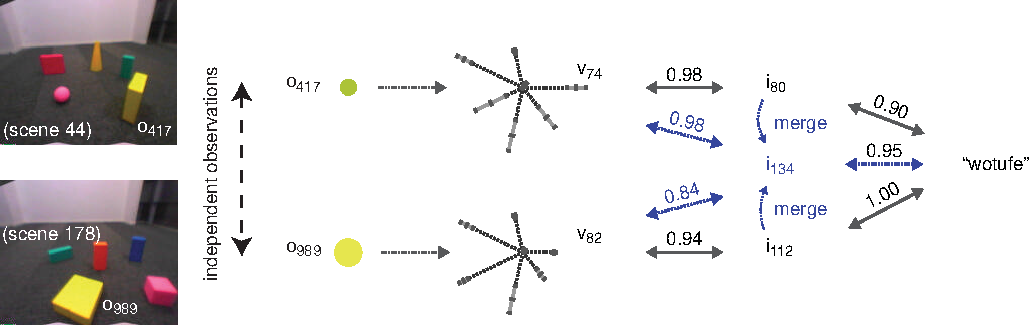
\includegraphics[width=1\textwidth]{figures/gng-heuristic-homonymy}
  \caption{The 'same name' heuristic. Independent experiences of
    different views of the yellow block have led to two separate
    prototypical views that are both connected to the homonymous word
    ``wotufe''. Assuming that individuals that have the same name must
    be about the same physical object, the connected individuals can be
    merged.}
  \label{f:gng-heuristic-homonymy}
\end{figure}

Agents that view a scene from different angles can have very different
perceptions of the same object due to shadows, different sides of the
object facing the camera, different distances to the robots, and so
on. Consequently, it can happen that a hearer adopts a name for a
different individual than if he would have perceived the scene from
the viewpoint of the speaker, creating a homonym as a result. This
information also can be used to optimize semiotic networks as
illustrated in figure \ref{f:gng-heuristic-homonymy}. An agent has
established stable links between the name ``wotufe'' and the
individuals $i_{80}$ and $i_{112}$ thus can assume that the connected
prototypical views $v_{74}$ and $v_{82}$ are about the same physical
object. Similar to the object tracking heuristic, the two individuals
get merged by rerouting existing network connections a new individual
$i_{134}$. As discussed in section \ref{s:gng-lexicon} above, homonymy
can also arise due to misaligned prototypes. That's why the merging
operation is only done when the name and the connected prototypes are
stable and successful, i.e. the connections to the original
individuals have a score higher or equal than 0.9.


\begin{figure}[t]
  \gnuplotfigure{figures/gng-results-with-homonymy-heuristic}
  \caption{Commun\-icative success (measure
    \ref{m:communicative-success}) and inventory sizes (measures
    \ref{m:lexicon-size}, \ref{m:number-of-prototypical-views} and
    \ref{m:number-of-individuals}) in agents that use the same name
    heuristic. }
  \label{f:gng-results-with-homonymy-heuristic}
\end{figure}


Agents that use this heuristic on average merge two pairs of
individuals, reducing their number form 17 to about 15 as shown in
figure \ref{f:gng-results-with-homonymy-heuristic}. The optimal level
of 10 individuals (compare figure
\ref{f:gng-results-with-object-tracking-heuristic}) is not reached
because the agents create only a small number of homonyms (see
figure \ref{f:gng-number-of-words-and-synonyms-and-homonyms}) when
interacting in the particular environment used in this experiment.
Communicative success is as high as in figure
\ref{f:gng-results-no-heuristics} ($>$95$\%$) because this way of
rearranging the semiotic network does not change the behavior of the
agent -- the homonymous names were used successfully before and
changing their internal structure does not change how they are used.


\section{Alignment dynamics}
\label{s:gng-dynamics}

\begin{figure}[t]
  \centerline{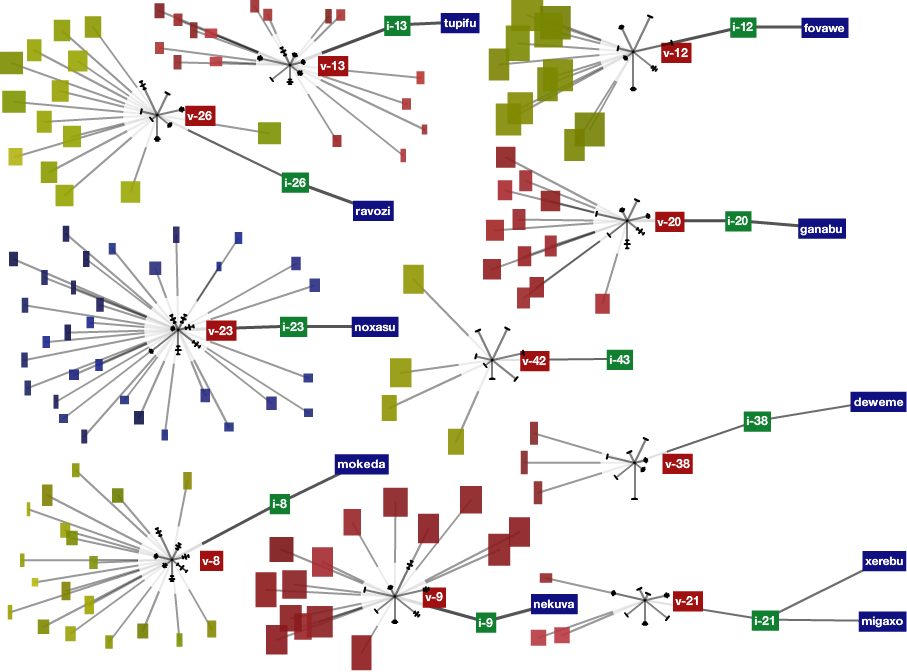
\includegraphics[width=\textwidth]{figures/gng-semiotic-network-example-1}}
  \caption{Visualization of a single agent's semiotic network after
    500 interactions. Words are represented as blue rectangles,
    individuals in green and prototypical views in red. The thickness
    of the connecting edges represents connection
    weights. Visualizations of past sensory experiences are drawn in
    their average color, width and height and are connected to the
    closest prototypical view with the smallest distance. Note that
    agents don't keep sensory experiences in memory -- here it is done
    for visualization purposes only.}
  \label{f:gng-semiotic-network-example-1}
\end{figure}

\begin{figure}[t]
  \centerline{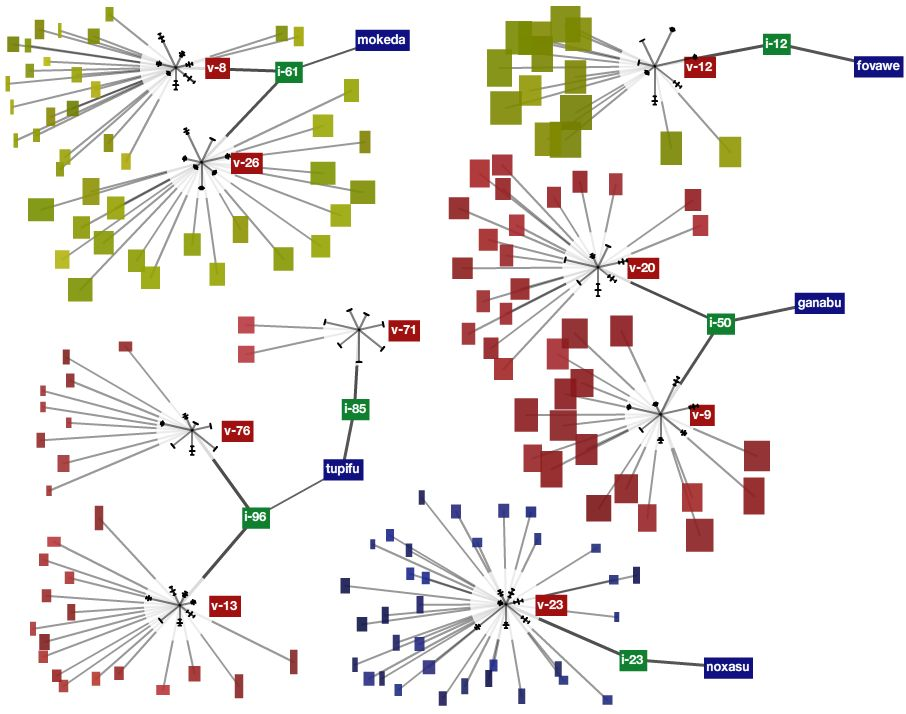
\includegraphics[width=1\textwidth]{figures/gng-semiotic-network-example-2}}
  \caption{The semiotic network of the same agent as in Figure
    \ref{f:gng-semiotic-network-example-1} after 10000 interactions.}
  \label{f:gng-semiotic-network-example-2}
\end{figure}

Agents that independently construct and align their semiotic networks
can self-organize successful communication systems and using
heuristics helps them to establish object identity. Figures
\ref{f:gng-semiotic-network-example-1} and
\ref{f:gng-semiotic-network-example-2} show an actual network of a
single agent after 500 and 10000 interactions. To keep the graphics
readable, the populations size was limited to 10 and a data set
consisting of only five different physical objects (three small blocks
in yellow, red, blue and two big boxes in yellow and red) was
used. 

After 500 interactions, this agent had created 10 different
prototypical with corresponding individuals -- among them two separate
ones for the small yellow block ($v_8$ and $v_{26}$), two for the big
yellow block ($v_{42}$ and $v_{12}$), two for the big red box
($v_{20}$ and $v_9$), and three for the small red block ($v_{76}$,
$v_{13}$ and $v_{71}$). 9500 interactions later, the prototypical view
$v_{42}$ disappeared from the semiotic network because its region in
sensory space was taken over by one of the other prototypical views
for yellow blocks. It was already not connected to a word form in
interaction 500 and consequently also not used and thus subsequently
removed to to the constant decay of prototype scores.

Using the object tracking heuristic, three pairs of prototypical views
got merged into individuals ($i_{61}$ for small yellow blocks,
$i_{96}$ for small red blocks and $i_{50}$ for big red boxes),
reducing their number to six. Finally, synonymy has been completely
dampened in this network and the homonymous name ``tupifu'' is stably
linked to the individuals $i_{96}$ and $i_{85}$, resulting in a
lexicon size of five names for five physical objects. When the series
of language games would have continued after interaction 10000, it
could have happened that the individuals $i_{85}$ and $i_{96}$ get
merged due to the ``same name'' heuristic.


\subsection{Crucial factors}

We don't claim that the particular mechanisms for maintaining semiotic
networks as introduced above are the only possible solution to the
problem of how a population of agents can self-organize a set of
individual names for physical objects. Many strategies (i.e. for the
adjustment of prototypical views, lexicon update, etc.) were tested to
improve measures such as communicative success and inventory
sizes. But other design choices seemed to have little impact on the
overall performance -- making the system robust in a wide range of
parameters. For example the model works well when using different
kinds of physical objects (different data sets, see section
\ref{s:recording-data-sets}), other sets of visual features, different
distance measures for nearest neighbor computation, other mechanisms
for damping synonymy, and generally different values for thresholds or
changes in updating scores.

\begin{figure}[p]
  \gnuplotfigure{figures/gng-update-stragegies-vs-success}
  \caption{The impact of three different strategies for updating the
    semiotic network on communicative success (see text). As a
    baseline, parameters and strategies are as discussed above and
    agents use the object tracking heuristic. Results are averaged of
    20 runs of 25000 language games.}
  \label{f:gng-update-stragegies-vs-success}
\end{figure}


\begin{figure}[p]
  \gnuplotfigure{figures/gng-update-stragegies-vs-lexicon-change}
  \caption{The influence of three different update strategies on
    lexicon change frequencies (how often agents add to or remove
    words from their lexicons, see measure
    \ref{m:frequency-of-lexicon-changes} on page
    \pageref{m:frequency-of-lexicon-changes}).}
  \label{f:gng-update-stragegies-vs-lexicon-change}
\end{figure}

\begin{figure}[p]
  \gnuplotfigure{figures/gng-update-stragegies-vs-number-of-prototypes}
  \caption{The average number of prototypical views in each agent's
    semiotic network for three different update strategies.}
  \label{f:gng-update-stragegies-vs-number-of-prototypes}
\end{figure}

However, three different strategies for updating semiotic networks
were found to be crucial for the dynamics of our model. Figures
\ref{f:gng-update-stragegies-vs-success}--\ref
{f:gng-update-stragegies-vs-number-of-prototypes} compare the
performance in agents that don't use these strategies with a baseline
condition (agents maintain their networks as discussed before and use
the object tracking heuristic). First, homonymy damping (similar to
the damping of synonyms, the scores of words with the same form but
different meanings are reduced after each successful interaction)
seems to destabilize the construction of semiotic networks. As
discussed above, agents sometimes successfully use the same name for
different individuals and the damping of homonymy would force them to
use different names instead. As a result, words are more often added
or removed (figure \ref{f:gng-update-stragegies-vs-lexicon-change})
and the number of prototypes is slightly higher than in the baseline
configuration (figure
\ref{f:gng-update-stragegies-vs-number-of-prototypes}) due to higher
fluctuations. This finding is interesting because in many other models
of embodied lexicon formation the damping of homonymy is crucial.

Second, it is important that agents keep words that reached zero score
in a separate memory. This prevents speakers from creating new names
all the time (it is still better to use a word that had little success
in the past than a completely new word because at least some of the
agents might know the word) and allows hearers to guess the meanings
of words even when their confidence in the names is low.  Agents not
memorizing words with zero score consequently reach much less
communicative success (figure
\ref{f:gng-update-stragegies-vs-success}) and maintain a lower, less
optimal number of prototypes (figure
\ref{f:gng-update-stragegies-vs-number-of-prototypes}) due to less
reinforcement from language. The frequency of lexicon changes is lower
(figure \ref{f:gng-update-stragegies-vs-lexicon-change}) because
re-adding a zero score word to the set of actively used connections or
removing a word from this set is also counted as a lexicon change.

Third, adjustment of prototypes (adapting their feature values to
better capture the statistical distribution of associated sensory
experiences) is crucial too. Agents not doing this will create less
prototypical views that are less representative for the objects
associated to them (see also figure \ref{f:gng-prototype-similarity},
page \pageref{f:gng-prototype-similarity}) and consequently reach less
communicative success (figure
\ref{f:gng-update-stragegies-vs-success}).


\subsection{Scaling with population size}

One of the most important properties of language evolution models is
how they scale with increasing population sizes -- and this one scales
very well. We ran populations of 10, 50, 100, 500 and 1000 agents that
use the object tracking heuristic and compared their performance
(figures \ref{f:gng-population-size-vs-success}--\ref
{f:gng-population-size-vs-lexicon-size}). Populations of different
sizes naturally require different numbers of language games to be
played for aligning their inventories: in order to make the results
comparable, values on the x-axis are not the usual absolute number of
language games played but the average number of interactions per
agent. Because always two agents take part in an interaction, the
number of interactions per agent is on average the absolute number of
interactions divided by half of the population size. Thus, 10 agents
played 25000 language games, 50 agents 125000 interactions, 100 agents
250000 and so on.

\begin{figure}[p]
  \gnuplotfigure{figures/gng-population-size-vs-success}
  \caption{Communicative success in populations of different sizes
    playing a population size dependent number of games. Results are
    averaged over 8 repeated runs each. Note that values along the
    x-axis are for the number of interactions played per agent (see
    text).}
  \label{f:gng-population-size-vs-success}
\end{figure}

\begin{figure}[p]
  \gnuplotfigure{figures/gng-population-size-vs-lexicon-changes}
  \caption{The impact of population size on the frequency lexicon
    changes over the average number of games played by each agent.}
  \label{f:gng-population-size-vs-lexicon-changes}
\end{figure}

\begin{figure}[p]
  \gnuplotfigure{figures/gng-population-size-vs-lexicon-size}
  \caption{The impact of population size on lexicon sizes plotted over
    the number of interactions per agent.}
  \label{f:gng-population-size-vs-lexicon-size}
\end{figure}

The same high level of success as in figure
\ref{f:gng-results-with-object-tracking-heuristic} is reached by
populations of all sizes (figure
\ref{f:gng-population-size-vs-success}), but reaching it takes the
longer the bigger the number of agents. This is due to the fact that
different speakers independently invent more names and thus the
alignment of names takes more interactions. The maximum lexicon size
before synonymy damping kicks in is about 25 in a population of 10
agents but $\approx$125 for 1000 agents (figure
\ref{f:gng-population-size-vs-lexicon-size}). Despite the different
number of synonyms introduced by populations of different sizes, their
lexicons remain equally stable once synonyms have been inhibited
(figure \ref{f:gng-population-size-vs-lexicon-changes}). The
remarkably good scaling of performance is explained with the fact that
the agents independently construct their inventories of prototypical
views and individuals (their size in fact remains the same for
different population sizes) -- the delay in communicative success for
bigger populations is mainly due the additional difficulty of aligning
the higher number of names.




%%% Local Variables: 
%%% mode: latex
%%% TeX-master: "phdbook"
%%% End: 
